\documentclass{fkssolpub}

\usepackage[czech]{babel}
\usepackage{fontspec}
\usepackage{fkssugar}
\usepackage{amsmath}
\usepackage{graphicx}

\author{Ondřej Sedláček}
\school{Gymnázium Oty Pavla} 
\series{1p}
\problem{1} 

\begin{document}

Víme, že největší počet trojúhelníků je $\binom{6}{3} = 20$. Tím pádem abychom dostali 17 nedegenerovaných trojúhelníků, musím body uspořádat tak, aby vznikli právě 3 degenerované trojúhelníky. Toho dosáhneme tak, že 3 různé trojice budou na jedné přímce, protože tehdy tyto trojice nemůžou vytvořit trojúhelník.

Teď už víme dost informací na to, abychom mohli rozmístit body. Jedno z možných řešení je níže:

\begin{figure}[h!]
	\begin{center}
		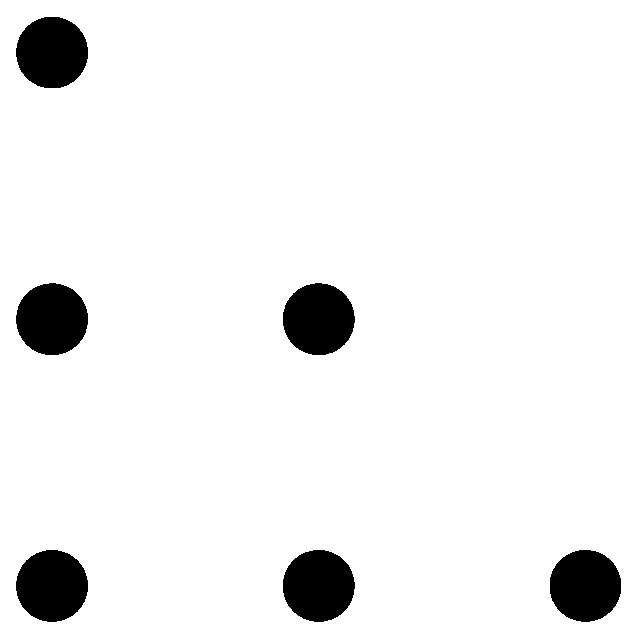
\includegraphics[width=0.50\textwidth]{1-fig.eps}
	\end{center}
	\caption{Jedno z možných řešení}
	\label{fig:}
\end{figure}


\end{document}
